Tässä luvussa esitetään perusteet ja tarvittavat tiedot hyväksymistestauksesta, johon testauksen tasoista tässä diplomityössä keskitytään.
Ensin esitetään hyväksymistestauksen tarkoitus, jonka jälkeen keskitytään hyväksymistestausvetoiseen kehitykseen ja sen esittelemiseen ohjelmistotuotannollisena menetelmänä.
Hyväksymistestausvetoisen kehityksen jälkeen käydään läpi web-sovelluksien yhteydessä huomioitavia erityispiirteitä hyväksymistestauksen toteuttamisen näkökulmasta.
Web-sovelluksien erityispiirteiden jälkeen esitetään tämän diplomityön yhteydessä kehitetyn hyväksymistestausjärjestelmän rakentamiseen käytettyjä, mutta kuitenkin myös hyvin yleisiä hyväksymistestauksen työkaluja.
Testausjärjestelmän rakenteen lisäksi käydään läpi myös testitapauksien rakentaminen painottuen testausjärjestelmässä käytettyihin työkaluihin.
Lopuksi esitetään testitapauksiin tärkeästi liittyvä priorisointiongelma, pyritään esittämään miksi sen ratkaiseminen on tärkeää, ja esitetään erilaisia menetelmiä sen ratkaisemiseen.

\section{Hyväksymistestauksen tarkoitus} \label{ch:08_hyvaksymistestauksen_tarkoitus}

  Hyväksymistestaus on yksi tärkeimmistä testauksen tasoista, sillä sen ollessa kattava, voidaan verifioida ohjelman toiminta korkealla tasolla saaden samalla varmuus siitä, että hyväksymistestausta alemmilla tasoilla testattavat asiat toimivat riittävän oikein.
  Hyväksymistestauksen tarkoituksena on varmistaa toteutettavan ohjelmiston vaatimusten toimivuus erityisesti käytännön tilanteissa siten, että voidaan varmistaa, vastaako ohjelmisto loppukäyttäjän tarpeita.
  Hyväksymistestaus antaa vastauksen siihen, toimiiko toteutettu järjestelmä loppukäyttäjän tarpeiden mukaisesti, ja loppukäyttäjän näkökulmasta oikein.
  Hyväksymistestauksen sanotaan olevan muodollista testaamista, jossa käyttäjän tarpeet, vaatimukset ja liiketoimintaprosessit otetaan huomioon selvittäessä, täyttääkö järjestelmä hyväksymisen kriteerit ja sallii auktorisoidun tahon päättää hyväksytäänkö järjestelmä julkaistavaksi \cite{istqb_glossary_v3_2}.
  Ohjelmistotestauksen tekniikoiden näkökulmasta hyväksymistestaus on mustalaatikkotestausta, eli testauskohdetta testataan tietämättä sen teknisestä toteutuksesta.
  Hyväksymistestauksen painoarvo on asiakasperusteisessa vaatimusmäärittelyssä ja loppukäyttäjän tarpeiden kartoittamisessa.
  Testiautomaation osalta hyväksymistestausta varten voidaan rakentaa testitapaukset, joiden avulla voidaan keskittyä varmistamaan loppukäyttäjille tarpeellisten toimintojen toteutuminen testitapauksien suorittamisen jälkeen.
  Hyväksymistestauksen osalta testitapauksia voidaan toteuttaa niin sanotulla päästä päähän -periaatteella, jossa testattavaa järjestelmää testataan siten kuin loppukäyttäjä sitä käyttäisi.
  Hyväksymistestauksessa ei anneta painoarvoa esimerkiksi kosmeettisille tai kirjoitusvirheille, vaan pyritään selvittämään loppukäyttäjille oleellisten ja tarpeellisten toimintojen toteutuminen.

  Hyväksymistestaus on luvussa \ref{ch:07_testauksen_tasot} esitetyistä testauksen tasoista viimeinen ja sen suorittamisen jälkeen saadaan tieto, onko järjestelmä toteutuksen osalta sellaisenaan valmis julkaistavaksi.
  Perinteisesti hyväksymistestauksen lähtökohtia ovat selvät hyväksymisvaatimukset sekä julkaisukelpoinen toteutus, joka voi sisältää vain kosmeettisia tai kirjoitusvirheitä.
  Hyväksymisvaatimukset voivat olla esimerkiksi liiketoiminnallisia käyttötapauksia, prosessivirtauskaavioita tai ohjelmiston vaatimusmäärittely.
  Testiautomaatiota varten käytettävästä testialustasta riippuen hyväksymistestauksen käyttötapaukset voidaan muodostaa joko osittain tai suoraan testitapauksiksi.
  Hyväksymistestaukseen usein pyydetään osallisiksi ohjelmistokehittäjien lisäksi myös muita sidosryhmiä, ja toisinaan jopa loppukäyttäjiä.
  Keskeistä on, että loppukäyttäjiltä hankitaan tieto tarvittavista ja toteutettavista ominaisuuksista, kun taas muut sidosryhmät kuten esimerkiksi johtoryhmä voivat tehdä liiketoiminnallisia päätöksiä hyväksymistestauksen onnistumisen osalta ja esimerkiksi peruuttaa julkaisun.
  Hyväksymistestaus siis antaa mahdollisuuden korjata usein liiketoiminnallisestakin näkökulmasta merkittävät toiminnalliset virheet ennen kuin järjestelmä julkaistaan loppukäyttäjille.

  Kehittäjien käsitys järjestelmän toiminnallisuudesta ja sen vaatimuksista voi kuitenkin olla usein hyvin erilainen kuin loppukäyttäjien.
  Hyväksymistestauksen avulla voidaan lievittää tätä ongelmaa, ja saada ohjelmistokehittäjät loppukäyttäjien kanssa vaatimusmäärittelyn suhteen samalle aaltopituudelle.
  Testiautomaation avulla toteutettavalla toistuvalla hyväksymistestauksella varmistetaan, että järjestelmä toteuttaa loppukäyttäjän tarpeet vielä järjestelmään tehtyjen muutoksien jälkeen.
  Hyväksymistestauksen testitapaukset heijastavat tarkoituksenmukaisesti suoraan loppukäyttäjien tarpeita, jonka avulla ohjelmistokehittäjät ja muut sidosryhmät voivat tehokkaasti varmistaa järjestelmän valmiuden ja senhetkisen tilan.
  Hyväksymistestauksella siis saadaan katsaus ohjelmiston valmiudesta sen vaatimuksiin ja loppukäyttäjien toiminnallisiin tarpeisiin nähden.

\section{Hyväksymistestausvetoinen kehitys} \label{ch:08_hyvaksymistestausvetoinen_kehitys}

  Hyväksymistestausvetoisen kehityksen tarkoituksena, kuten myös testausvetoisessa kehityksessä, on toteuttaa ohjelmistotuotannollinen prosessi laatien toistettavasti suoritettavat testitapaukset ennen ohjelmiston varsinaista toteutusta.
  Hyväksymistestausvetoisessa kehityksessä tämä tarkoittaa käytännössä sitä, että ennen toteutusta luodaan tarvittavat ohjelmiston asiakasvaatimuksia palvelevat hyväksymistestit, jotka ohjelmiston on tarkoitus läpäistä sen julkaisemisen hyväksymiseksi.
  Hyväksymistestausvetoisen kehityksen sanotaan olevan yhteistyöhön perustuva lähestymistapa kehitykseen, jossa tiimi ja asiakkaat käyttävät asiakkaiden oman ympäristön kieltä ymmärtääkseen heidän vaatimukset, jotka muodostavat pohjan komponentin tai järjestelmän testaamiseen \cite{istqb_glossary_v3_3}.
  Tarvittavat ohjelmiston hyväksymistestit suoritetaan iteratiivisesti ohjelmistokehitysprosessin aikana ja se tarkoittaa käytännössä jatkuvan integraation ottamista käyttöön ohjelmistokehityksessä.
  Hyväksymistestausvetoinen kehitys on erittäin hyödyllinen ohjelmistokehityksessä käytetty menetelmä, sillä kehitysvaiheessa on aina tarkasti tiedossa, vastaako ohjelmiston senhetkinen tila asiakasvaatimuksia, ja kuinka hyvin se niiden täyttämisessä onnistuu.

  \begin{figure}[H]
    \centering
    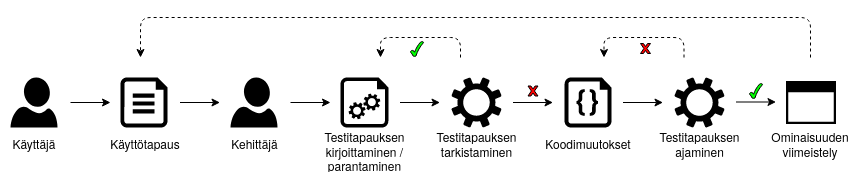
\includegraphics[width=0.8\textwidth]{assets/hyvaksymistestausvetoinen-kehitys.png}
    \caption{Hyväksymistestausvetoisen kehityksen vaiheet \parencite{atdd_steps}}
    \label{fig:hyvaksymistestausvetoinen-kehitys}
  \end{figure}

  Hyväksymistestausvetoinen kehityksen vaiheet on esitetty kuvassa \ref{fig:hyvaksymistestausvetoinen-kehitys}, josta voidaan huomata sen olevan testausvetoisen kehityksen kanssa pääpiirteittäin hyvin samanlainen, mutta ennen ohjelmistokehityksen aloitusta asiakasvaatimukset kartoitetaan ja ohjelmiston hyväksyttävyys määritellään.
  Hyväksymistestitapaukset kirjoitetaan testausvetoisen kehityksen mukaisesti ennen toteutusta ja ohjelmistokehitys itsessään noudattaa iteratiivisesti testausvetoista kehitystä, vaikka hyväksymistestaus on perinteisesti vaatinut lähes valmista järjestelmää \parencite{traditional_acceptance_testing}.
  Asiakasvaatimukset määritetään usein käyttötapauksien muodossa ja hieman testialustasta riippuen ne voidaan kirjoittaa suoraan testitapauksien muotoon.
  Hyväksymistestausvetoisessa kehityksessä ohjelmistokehitystä ohjaavat asiakasvaatimukset ja loppukäyttäjien tarpeiden toteutuminen, jotka ovat hyvin usein toiminnallisia vaatimuksia.
  Hyväksymistestausvetoisessa kehityksessä mitataan jatkuvasti käyttötapauksien muodossa validoitavien haluttujen ominaisuuksien toteutumista.
  Perusperiaate on kirjoittaa asiakasvaatimus tai käyttötapaus testitapauksen muotoon, toteuttaa testitapaus, ajaa testitapaus läpäisemättömänä, toteuttaa ominaisuus, ajaa testitapaus läpäisevänä, refaktoroida toteutus ja siirtyä takaisin seuraavaan käyttötapaukseen.
  Käyttötapaus koostuu rakenteellisesti usein tilanteesta, motivaatiosta ja halutusta lopputuloksesta.
  Esimerkki käyttötapauksesta voi olla: \emph{käyttäjänä, haluan sisäänkirjautumisen jälkeen voida avata premium-ominaisuudet tekemällä sovelluksensisäisen oston}.

  Hyväksymistestausvetoisessa kehityksessä hyväksymistestit on hyödyllistä pilkkoa pieniin hallittaviin kokonaisuuksiin, jolloin voidaan iteratiivisesti toteuttaa valmiiksi tietyn testitapauksen mukainen ominaisuus, joka vastaa jotakin käyttötapausta tai loppukäyttäjän tarvetta.
  Hyväksymistestauksessa testitapaus voi olla esimerkiksi käyttäjän tietojen muuttumisen varmistaminen, kuten tason läpäiseminen pelisovelluksessa, joka muuttaa käyttäjän edistystä.
  Menetelmänä hyväksymistestausvetoisen kehityksen tarkoituksena on onnistua vastaamaan loppukäyttäjän tarpeisiin tehokkaasti ja hyvin ottamalla tarpeet huomioon jo ennen toteutuksen aloittamista.
  Menetelmän avulla myös luodaan ymmärrystä ohjelmistotuotteen valmiuden määritelmästä, kun eri sidosryhmät voidaan saada sen suhteen samalle aaltopituudelle.
  Hyväksymistestausvetoinen kehitys on lisäksi erittäin hyödyllistä, sillä jatkuva testaaminen antaa mahdollisuuden haluttujen ominaisuuksien toteutumisen validoimiselle menetelmän jokaisen iteraation koontiversiossa.

\section{Web-sovelluksien erityispiirteet} \label{ch:08_websovelluksien_erityispiirteet}

  Web-sovelluksilla on omia erityispiirteitä, jotka vaikuttavat testitapauksien laatimiseen.
  Nykypäivänä web-sovellukset ovat kasvaneet kompleksisuudessa ja front-end -puolen toteutuksia tarkasteltaessa web-sovellukset usein muistuttavat jo perinteisiä, dynaamisia työpöytäsovelluksia.
  Web-sovelluksia päivitetään usein niin tiheään tahtiin, jotta niille on suuri tarve luoda testiautomaatiota, jota hyödyntäen voidaan varmistaa, että ne toimivat oikein myös muutosten jälkeen.

  Hyväksymistestauksen priorisoimisen osalta tärkeä web-sovelluksien erityispiirre liittyy käyttöliittymiin ja DOM-dokumenttiobjektimalliin.
  Dokumenttiobjektimallin avulla verkkoselaimet esittävät käyttöliittymän ja siinä näkyvän sisällön.
  Tämän lisäksi dokumenttiobjektimalli mahdollistaa käyttöliittymässä olevien elementtien valitsemisen, jota hyödynnetään vahvasti testitapauksien kirjoittamisessa.

  Navigointi ja navigointiketjut ovat myös yksi web-sovelluksien erityispiirre.
  Historiallisesti verkkosivuilla navigointi tapahtuu niin sanottujen hyperlinkkien avulla, verkkosivujen itse ollessa hypertekstiä.
  Tämä historiallinen lähestymistapa on edelleen käytössä ja web-sovelluksissa on lähes poikkeuksetta useita hyperlinkkejä, joiden avulla navigoiminen luo navigointiketjuja, joissa edelliseen sivuun tiedetään palata.
  Hyperlinkkien avulla tapahtuva navigointi ja navigointiketjut ovat sellainen erityispiirre, jotka on hyvä tiedostaa myös hyväksymistestauksen testitapauksia rakentaessa.

  Web-sovelluksien syötteet ja niiden yhteyteen liittyvä tietoturva ovat erityispiirre joka vaatii suurta huomiota.
  Web-sovelluksien syötteisiin on perinteisesti liittynyt paljon haavoittuvuuksia, kuten esimerkiksi XSS-hyökkäykset ja SQL-injektiot.
  Web-sovelluksien hyväksymistestauksen testitapauksiin on hyvä sisällyttää syötteisiin liittyvää testaamista, joissa tietoturva pidetään mielessä.

  Erilaisia web-sovelluksen loppukäyttäjien asiakasympäristöjä on erittäin paljon, mikä kannustaa moniselaimellisen testauksen rakentamiseen.
  Näissä ympäristöissä on omat verkkoselaimet, näyttöresoluutiot ja selainasetukset, jotka saavat saman web-sovelluksen toimimaan eri tavoilla eri ympäristöissä, ja luovat siten usein jopa päänvaivaa ohjelmistokehittäjille.
  Etenkin web-käyttöliittymiin keskittyessä testitapauksiin on hyvä sisällyttää erilaisia näyttöresoluutioita, ruudunkaappauksien ottamista ja selainasetuksia, kuten esimerkiksi JavaScript-ominaisuuksien estäminen.

  Web-sovelluksien käyttöliittymien testaaminen, ja yleisesti ottaen kaikenlaisten käyttöliittymien testaaminen, on perinteisesti tapahtunut manuaalisesti.
  Nykyään web-sovelluksia voidaan testata niin sanotun päätteettömän testauksen keinoin.
  Web-sovelluksien päätteettömässä testauksessa verkkoselaimen, näyttöresoluution ja selainasetuksien muodostama asiakasympäristö rakennetaan virtualisoinnin avulla.
  Virtualisoinnista vastaa joko verkkoselaimet itse tai siihen voidaan käyttää käyttöjärjestelmätasolla näyttöpalvelimen protokollan toteuttavaa virtualisointiratkaisua.
  Virtualisoitu asiakasympäristö rakennetaan siten, että se päätteettömänä vastaa täysin päätteellistä vaihtoehtoa ja siitä voidaan ottaa esimerkiksi ruudunkaappauksia, vaikka mitään ihmisen aistittavaa ei olisikaan näkyvillä.

\section{Hyväksymistestausjärjestelmä} \label{ch:08_hyvaksymistestausjarjestelma}

  Tässä kappaleessa esitetään diplomityötä tehdessä käytettyjä ja osin myös varsin yleisiä testiautomaation mahdollistavia työkaluja, kukin omassa alakappaleessaan.
  Ensin esitetään hyväksymistestauksen automatisoimisen kannalta kaikista tärkeimmät työkalut, eli testialustana käytettävä Robot Framework ja web-sovelluksien kanssa vuorovaikuttamisen automatisoimisen mahdollistava Selenium-kirjasto.
  Lisäksi esitetään kolme muuta tärkeää työkalua, joiden avulla voidaan rakentaa kokonainen ohjelmistotuotannon prosessiin integroitavissa oleva hyväksymistestausjärjestelmä.
  Toteutuksessa GoCD vastaa jatkuvan integroinnin tarjoamisesta, Xvfb vastaa päätteettömän testauksen tarjoamisesta ja Docker vastaa työkalujen virtualisoimisesta ja säiliöinnistä, jolloin työkaluista saadaan rakennettua yhtenäinen kokonaisuus.
  Tämän diplomityön tuloksena syntynyt hyväksymistestausjärjestelmä koostuu samoista työkaluista kuin seuraavissa kappaleissa on esitetty.

  \subsection{Robot Framework} \label{ch:08_robot_framework}

    Robot Framework on geneerinen avoimen lähdekoodin testialusta hyväksymistestaukseen, hyväksymistestausvetoiseen kehitykseen ja robottisten prosessien automaatioon \parencite{robot_framework_user_guide}.
    Robot Frameworkin avainsanaperusteinen syntaksi on helposti ymmärrettävä, luettava ja selkeä.
    Testialustan etuna on helppo lähestyttävyys, eikä sen päälle rakennettujen testitapauksien ymmärtäminen vaadi ohjelmointikielten ymmärtämistä.
    Robot Framework on Python-ohjelmointikieleen perustuva testialusta ja se on helppo asentaa, sitä on helppo ymmärtää, sillä on kattava dokumentaatio ja se on helppoa ottaa käyttöön.

    Robot Frameworkissa on sisäänrakennettu tuki ulkoisille kirjastoille, jota havainnollistetaan kuvassa \ref{fig:robot-architecture}, ja sen kattavasta dokumentaatiosta löytyy tietoa omien avainsanojen ja omien kirjastojen tekemiseen.
    Lisäksi Robot Framework on todella suosittu testialusta, mikä näkyy muun muassa siitä, että sisäänrakennettujen ominaisuuksien lisäksi ulkoisia kolmansien osapuolien kirjastoja löytyy alustalle paljon.
    Robot Framework tukee muuttujien käyttöä testitapauksien rakentamisessa, joilla voi hieman lisätä kompleksisuutta ja logiikkaa omiin testitapauksiin.
    Robot Frameworkista löytyy myös tuki dataperustaisten testitapauksien rakentamiseen, joille annetaan eri syötteitä sisältävää testidataa.
    Testitapauksia voi myös ryhmitellä testikokoelmiin käyttämällä tägejä testitapauksien sisällä.

    \begin{figure}[H]
      \centering
      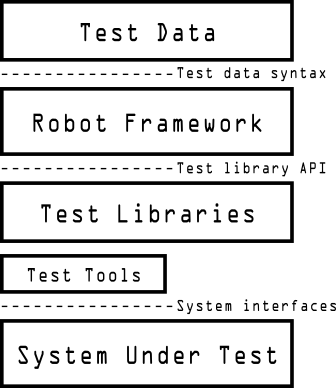
\includegraphics[width=0.6\textwidth]{assets/robot-arkkitehtuuri.png}
      \caption{Robot Framework alustan arkkitehtuuri \parencite{robot_framework_user_guide}}
      \label{fig:robot-architecture}
    \end{figure}

    Robot Frameworkillä rakennettuja testitapauksia voidaan ajaa komentoriviltä sen tarjoamalla robot-komennolla.
    Testitapauksien ajaminen tulostaa komentoriville yksinkertaisen raportin testitapauksen onnistumisesta, ja lisäksi tallettaa varsin yksityiskohtaisen ja selkeän testitaportin ajetuille testitapauksille.
    Testiraportit ovat erittäin hyvin tehtyjä ja HTML-pohjaisia, mikä tarkoittaa, että ne voidaan helposti integroida osaksi jatkuvan integraation koontiputkia.

    Yhtenä heikkoutena Robot Frameworkissa on tuen puuttuminen ohjelmistokieliä hyödyntävillä testialustoilla löytyville kontrollirakenteille, joita esiintyy esimerkiksi yksikkötestaukseen tarkoitetuilla testialustoilla.
    Robot Framework on selkeästi vain hyväksymistestauksen testitapauksien rakentamista varten tarkoitettu testialusta, ja sellaisenaan erinomainen vaihtoehto testitapauksien rakentamiseen.

  \subsection{Selenium} \label{ch:08_selenium}

    Selenium on suosittu avoimen lähdekoodin työkalu ja kirjastokokoelma verkkoselainten automatisoimiseen.
    Ensisijaisesti se on tarkoitettu web-sovelluksien automatisoimiseen testaustarpeita varten.
    Erityisen hyvin Selenium soveltuu hyväksymistestauksen testiautomaation rakentamiseen, sillä sen avulla automatisoidaan web-sovelluksien käyttöliittymissä tehtäviä toimenpiteitä.
    Selenium on ThoughtWorks-yhtiön kehittämä verkkoselainten automatisoimiseen tarkoitettu työkalujen ja kirjastojen kokoelma, ja se on saatavilla Windows, Linux ja MacOS -käyttöjärjestelmille \parencite{selenium_info_1}.
    Sama yhtiö on toteuttanut myös tässä diplomityössä myöhemmin esitettävän GoCD-ohjelmiston, jota voidaan käyttää jatkuvan integroimisen ja julkaiseminen rakentamiseen.

    Selenium-tuoteperheeseen kuuluvat Selenium WebDriver, Selenium IDE ja Selenium Grid -komponentit \parencite{selenium_info_2}.
    Selenium WebDriver on varsinainen web-sovelluksien automatisoimiseen käytettävä ohjelmisto, ja sitä käytetään myös tässä diplomityössä.
    Selenium IDE on ohjelmistokehittäjille ja testaajille tarkoitettu kehitysympäristö, jota voidaan halutessaan käyttää testitapauksien rakentamiseen.
    Selenium Grid on järjestelmä, jonka avulla voidaan Selenium pohjaisten testitapauksien suorittaminen hajauttaa skaalautuvasti useille eri etäkoneille.
    Tässä diplomityössä ei ole käytetty Selenium Grid -järjestelmää, vaan testitapauksien suorittamiseen tarvittavat ohjelmistot on säiliöity Docker-työkalua käyttäen, mikä mahdollistaa tarvittaessa skaalautuvuuden.

    Selenium on todella tärkeä osa web-sovelluksien testiautomaation rakentamista, sillä se pohjimmiltaan mahdollistaa web-sovelluksien käyttöliittymien käsittelemisen automatisoidusti.
    Selenium-työkalua voidaan käyttää erityisesti hyväksymistestauksen testitapauksien automatisoimiseen suoraan Selenium IDE:n avulla nauhoittaen testitapauksia tai kirjoittaen ne Selenium-skriptauskielellä.
    Selenium on joustava työkalu ja se tarjoaa Selenium Client API -rajapinnan, jonka avulla sitä voidaan käyttää muistakin ohjelmointikielistä, kuten C\#, JavaScript tai Python.

    Tässä diplomityössä Selenium-työkalua käytetään Robot Frameworkin yhteyteen integroituna ulkoisena kirjastona.
    Robot Frameworkille on saatavilla SeleniumLibrary-niminen kirjasto, josta löytyy Robot Frameworkin syntaksin mukaisesti määritellyt avainsanat verkkoselainten ohjaamiseen Selenium-pohjaisesti.

  \subsection{Xvfb} \label{ch:08_xvfb}

    Xvfb, eli X Virtual Framebuffer, on X-näyt\-tö\-pal\-ve\-li\-men  protokollan toteuttava virtuaalinen X-näyt\-tö\-pal\-ve\-lin.
    X-näyt\-tö\-pal\-ve\-li\-men tehtävä on mahdollistaa graafisten ohjelmien toiminta käyttöjärjestelmän ytimen päällä, jossa X-palvelin ja X-asiakasohjelmat kommunikoivat keskenään. Lisäksi X-palvelin hoitaa ytimen kautta näytön ja syöttölaitteiden käsittelyn.
    Xvfb ei tulosta mitään näytölle, vaan kaikki näytölle normaalisti tulostuva graafisia käyttöliittymiä sisältävä sisältö on ajonaikaisessa tietokoneen muistissa.
    Xvfb toimii aivan kuten tavallinen X-näyt\-tö\-pal\-ve\-lin, eli vastaa X-ohjelmien pyyntöihin ja hoitaa niihin liittyvän tapahtumien ja virheiden käsittelyn.

    Xvfb soveltuu web-sovelluksien hyväksymistestauksen automatisointiin mahdollistaen päätteettömän testaamisen testitapauksille.
    Päätteetöntä testausta voidaan toteuttaa myös verkkoselaimiin rakennettujen ominaisuuksien avulla, mutta Xvfb:n suurena etuna niihin verrattuna on se, että sitä voidaan käyttää mihin tahansa graafiseen ohjelmaan.
    Päätteettömän testauksen mahdollistaminen on erittäin tärkeää, sillä se mahdollistaa myös käyttöliittymätestauksen suorittamisen jatkuvan integroinnin palvelimilla, jossa graafista ympäristöä ei ajon aikana muuten olisi.

    Yksi Xvfb:n heikkouksista on, että se on saatavilla vain UNIX-pohjaisiin X-näyt\-tö\-pal\-ve\-li\-men sisältäviin käyttöjärjestelmiin, kuten Linux ja MacOS.
    Näin ollen esimerkiksi Windows-alustalla toimivaa Internet Explorer -verkkoselainta ei voida natiivisti testata.

    Robot Frameworkille on saatavilla XvfbRobot-niminen kirjasto, jota tämän diplomityön toteutuksessa käytettiin.
    XvfbRobot on kirjasto, josta löytyy Robot Frameworkin syntaksin mukaisesti määritellyt avainsanat Xvfb-palvelimen kanssa kommunikoimiseen.

  \subsection{Docker} \label{ch:08_docker}

    Docker on säiliöintityökalu, jonka avulla on mahdollista määrittää, rakentaa ja ajaa säiliöiden muotoon konfiguroituja sovelluksia.
    Docker muistuttaa virtuaalikoneita, mutta se on kevyempi ja resurssien käytössä optimaalisempi, sillä se jakaa käyttöjärjestelmän ytimen eri säiliöiden kesken ja virtualisoi vain sovellusympäristön, jonka säiliön määrittävä konfiguraatio sisältää, kuten kuvassa \ref{fig:docker-vs-virtual-machine} tarkemmin esitetään.
    Säiliöiden sisään voidaan paketoida kaikki kokonaisen sovelluksen tarvitsemat ohjelmistot, kirjastot, ympäristöt, riippuvuudet ja itse sovelluksen ohjelmakoodi.
    Rakentamalla säiliön ja käynnistämällä sen, voidaan sitä käyttää konfiguraatioltaan samanlaisena eri ympäristöissä, joissa Docker-ohjelmisto on saatavilla.

    \begin{figure}[H]
      \centering
      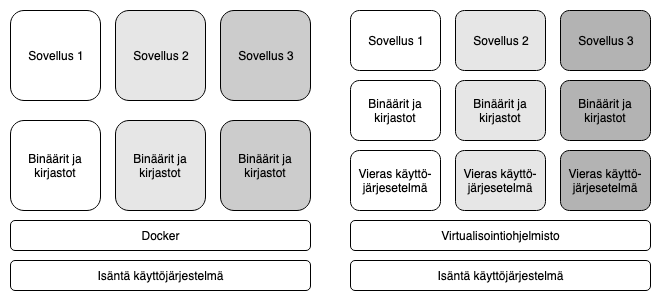
\includegraphics[width=0.8\textwidth]{assets/docker-vs-virtual-machine.png}
      \caption{Dockerin ja virtuaalikoneen arkkitehtuurivertailu \parencite{docker_vs_virtual_machine}}
      \label{fig:docker-vs-virtual-machine}
    \end{figure}

    Dockerfilen, eli Docker-säiliön kuvan konfiguraatiotiedoston, avulla voidaan luoda räätälöity säiliö, josta voidaan rakentaa yksi tai useampia säiliöinstansseja.
    Räätälöidyn säiliön etuna on etenkin se, että sen avulla saadaan aikaan sovellus, joka on periaatteessa alustasta riippumaton.
    Docker-ohjelmiston avulla sovelluskehittäjät voivat käyttää samaa Docker-konfiguraatiota rakentaakseen identtisiä säiliöitä sovelluskehityksen ajaksi.
    Tämän lisäksi Docker mahdollistaa saman Docker-konfiguraation käyttämisen sovelluksen pystyttämiseen ja julkaisemiseen nopeasti, helposti sekä jopa kustannustehokkaasti eri paikkoihin.
    Docker-compose on tapa rakentaa Docker-verkko, joka koostuu palveluista, jotka ovat joko valmiiksi tehtyjä Docker-kuvia tai itse Dockerfilen avulla tehtyjä Docker-säiliöiden kuvia.
    Docker-verkkoon voidaan myös lisätä yhteisiä tietosäilöjä, joita verkkoon kuuluvat palvelut voivat yhteisesti hyödyntää.
    Yksittäisen säiliön konfiguraation sisältämä Dockerfile ja kokonaisen Docker-verkon konfiguraation sisältämä Docker-compose -tiedosto kirjoitetaan YAML-kielellä.

    Tässä diplomityössä Dockeria käytettiin hyväksymistestauksen testitapauksien automatisoimiseen tarvittavien työkalujen säiliöinnissä.
    Olemassa olevaan Docker-verkkoon lisättiin hyväksymistestauksen testitapauksia varten tarkoitettu säiliö, joka hyödyntää Robot Frameworkiä, Seleniumia, Xvfb:ää, ja sisältää muun muassa testauksessa tarvittavat verkkoselaimet.
    Dockeria käyttämällä pystyttiin luomaan monistettava ja uniikki hyväksymistestauksen automatisointiympäristö, jota voidaan käyttää jatkuvan integraation yhteydessä testitapauksien suorittamiseen.

  \subsection{GoCD} \label{ch:08_gocd}

    GoCD on avoimen lähdekoodin jatkuvan integroinnin ja jatkuvan julkaisemisen mahdollistava palvelinohjelmisto.
    Ohjelmisto mahdollistaa koko koonti-testaus-julkaisu-putkiryhmän tai vain sen osien automatisoimisen.
    GoCD-palvelimen mainostetaan soveltuvan hyvin erityisesti jatkuvan julkaisemisen rakentamiseen.
    Myös GoCD on ThoughtWorks-yhtiön kehittämä ohjelmisto, kuten aiemmin esitetty Selenium-työkalukin \parencite{gocd_info}.

    Koonti-testaus-julkaisu-putkiryhmän voi rakentaa GoCD-palvelimen graafisen käyttöliittymän kautta tai koodina käyttäen YAML tai JSON-syntaksia.
    Teknisesti GoCD-ohjelmisto koostuu itse palvelimesta ja agenteista, jotka voivat suorittaa palvelimen pyytämänä ennalta määritettyjä koonti-testaus-julkaisu-putkiryhmän tehtäviä.
    Agentit on tarkoituksenmukaista sijoittaa eri järjestelmään kuin missä itse palvelin sijaitsee, ja agenteille voi määrittää resurssiominaisuuksia, jotka kertovat palvelimelle, mitä tehtäviä agenteilla voi teettää.
    GoCD-ohjelmiston terminologia on hieman tavallisesta poikkeavaa ja erilainen esimerkiksi todella suositun Jenkins-ohjelmiston vastaavista \parencite{gocd_jenkins_terminology}.
    GoCD-terminologiassa ylin käsite on putkiryhmä, jonka avulla yhteen kuuluvat putket voidaan järjestää samaan kokonaisuuteen.
    GoCD-terminologiassa yksittäinen putki vastaa esimerkiksi koonti- tai testausvaihetta.
    Yksittäisen putken alaisuudessa on vaiheita, jotka antavat GoCD-palvelimen käyttöliittymässä tiedon vaiheen onnistumisesta.
    Vaiheet itsessään sisältävät vielä tehtäviä, jotka ovat yksittäisiä komentoja tai sellaisia suoritettavia tehtäviä, jotka agentit pystyvät käsittelemään.
    GoCD-ohjelmiston terminologiaan kuuluvat vielä vahvasti artefaktit, jotka ovat sellaisia tiedostoja, mitä tehtävien suorittamisen yhteydessä syntyy, ja jotka on merkitty säästettäväksi.
    Esimerkkejä artefakteista ovat ohjelman koontiversiot tai testiraportit.

    Jatkuvan integraation yhteydessä tapahtuvan testiautomaation puolesta ei välttämättä ole suurta merkitystä sillä, mikä jatkuvan integraation mahdollistava palvelinohjelmisto on käytössä.
    Tämä havainto tuli esiin, kun tätä diplomityötä varten testiautomaatioon tarvittavat ohjelmistot säiliöitiin aiemmin esitetyllä Docker-työkalulla, jota voidaan yhden testausvaiheen tehtävän aikana kutsua komentorivipohjaisesti.

\section{Testitapauksien rakentaminen} \label{ch:08_testitapauksien_rakentaminen}

  Testitapaus on testiautomaation näkökulmasta määritelty toimenpiteiden, ehtojen ja muuttujien joukko, joka suorittamalla voidaan verifioida jokin osa, ominaisuus tai toiminnallisuus ohjelmistosta.
  Testitapauksien rakentaminen on järkevää järjestää testikokoelmiksi, jotka tarkoittavat samaan kontekstiin kuuluvista testitapauksista muodostettua joukkoa.
  Tässä diplomityössä esitettävään hyväksymistestaukseen liittyen testitapaukset kirjoitetaan usein käyttötapauksien muodossa.
  Hyväksymistestauksen tapauksessa testitapauksien määrittäminen testiautomaatiota varten voidaan toteuttaa Robot Frameworkillä ja apuna voidaan käyttää muita aiemmin mainittuja työkaluja.
  Lisäksi hyväksymistestauksen priorisoimiseen painotetun verkon avulla on välttämätöntä suunnitella ja rakentaa testitapaukset näkymä- ja siirtymäperusteisesti, koska menetelmä hyödyntää matemaattisia näkymä- ja siirtymäperusteisesti laadittuja painotettuja verkkoja.
  Terminä näkymä- ja siirtymäperusteisuus tarkoittaa yksinkertaisesti web-käyttöliittymien hyväksymistestauksessa yksittäisiä käyttöliittymän näkymiä ja niiden välisiä siirtymiä.
  Yleisiä web-käyttöliittymien näkymiä ovat esimerkiksi kirjautumisnäkymä, päänäkymä ja asetusnäkymä joiden välillä käyttäjät voivat siirtymä näkymästä toiseen.

  Testitapauksen perusformaatti koostuu lähtötilanteesta, laukaisijasta ja verifikaatiosta.
  Lähtötilanteessa tehdään olettamus ja seuraavassa vaiheessa seurataan, kun jokin ehto tapahtuu, minkä jälkeen voidaan tarkistaa seuraus ja verifioida onko se oletuksen mukainen.
  Perinteisesti hyvän testitapauksen on nähty koostuvan neljästä sen laatuun vaikuttavasta ominaisuudesta, jotka ovat virheiden havaitsemisen tehokkuus, esimerkillisyys eli kyky testata useita asioita samaan aikaan, taloudellisuus ja mukautumiskyky \cite[s.~4]{software_test_automation_book}.

  Robot Frameworkin perustaja on lisäksi kirjoittanut laajan ohjeistuksen siitä, miten Robot Frameworkiä käyttäen luodaan hyviä testitapauksia \cite{robot_framework_good_test_cases}.
  Klärckin ohjeistuksen pohjalta on huomioitava erityisesti testikokoelmien, testitapauksien ja avainsanojen nimeäminen, jonka kuuluisi olla selkeää, kuvaavaa ja ytimekästä.
  Dokumentaation määrää testitapauksissa tulisi rajoittaa, sillä hyvin kirjoitetut testitapaukset ovat Robot Frameworkiä käyttäen selkeitä jo sellaisenaan.
  Dokumentaatiota kuuluisi lisätä lähinnä vain testikokoelmiin yleisellä tasolla.
  Testikokoelmien kuuluisi sisältää vain toisiinsa liittyviä testejä, ja testitapauksien sekä avainsanojen tulisi olla sellaisenaan selkeästi ymmärrettäviä.
  Muuttujien käytöllä suositellaan kapseloimaan pitkiä ja kompleksisia arvoja, mutta arvojen syöttäminen ja palauttaminen muuttujia hyödyntäen tulisi pitää pois testitapauksien tasolta.

\section{Priorisointiongelma} \label{ch:08_priorisointiongelma}

  Testitapauksien priorisointi on kustannussyistä tai resurssien optimoinnin kannalta erittäin tärkeää.
  Ohjelmistotestauksessa on myös hyvä tiedostaa, että ohjelmistotuotetta ei usein voida testata täydellisesti, mikä nostaa esiin tarpeen tärkeimpien testitapauksien priorisoimisesta.
  Priorisoinnin toteuttamisen tärkeys korostuu erityisesti silloin, kun kohdejärjestelmä on kompleksinen ja toiminnallisia ominaisuuksia on paljon.
  Priorisointi vaatii kuitenkin priorisointimenetelmästä riippumatta ylimääräistä työtä ohjelmistokehittäjiltä ja -testaajilta.

  Priorisointiongelmaa voidaan ajatella sen laiminlyömisestä seuraavien haittojen näkökulmasta.
  Ilman testitapauksien priorisointia voi esiintyä muun muassa seuraavia haittoja.
  Prioriteettien puuttumisen seurauksena tärkeät ongelmat voidaan havaita vasta liian myöhään.
  Testitapauksia ei voida järjestää prioriteettien mukaan suoritettaviksi.
  Prioriteettijärjestyksen puuttumisesta johtuen epäoleellisten testitapauksien mukaan katkeava testaus voi piilottaa oleellisia testitapauksia.
  Tämän lisäksi myös prioriteettien puolesta epäoleelliset testitapaukset toteutetaan.
  Epäoleellisten testitapauksien toteuttaminen puolestaan kuluttaa resursseja ja lisää kustannuksia.
  Ajan myötä ohjelmistot ja niiden testaukseen toteutetut testitapaukset muuttuvat ja vanhenevat.
  Prioriteettien puuttuminen poistaa mahdollisuuden varautua oleellisten testitapauksien huolellisempaan ja aikaa kestävään suunnitteluun.
  Lisäksi testikattavuutta ei voida optimoida vähentämällä täysin epäoleellisia testitapauksia, jos niitä varten ei ole tehty priorisointia ennen toteutusta.

  Priorisointiongelman ratkaisemiseksi on olemassa useita erilaisia lähestymistapoja ja menetelmiä, kuten esimerkiksi heuristinen priorisointi tai MoSCoW-menetelmä.
  Tässä diplomityössä esitetään ja käytetään priorisointiin kuitenkin vain matemaattista, painotettuihin verkkoihin perustuvaa lähestymistapaa, joka on uudenlainen, tässä diplomityössä esitettävä, matemaattinen menetelmä priorisointiongelman ratkaisemiseen.
